\documentclass[12pt]{article}
\usepackage{a4wide,amssymb,epsfig,latexsym,multicol,array,hhline,fancyhdr}
\usepackage[utf8]{vietnam}
\usepackage[vietnamese,english]{babel}
\usepackage{amsmath}
\usepackage{lastpage}
\usepackage[lined,boxed,commentsnumbered]{algorithm2e}
\usepackage{enumerate}
\usepackage{color}
\parindent 0pt
\usepackage{graphicx}							% Standard graphics package
\usepackage{array}
\usepackage{float}
\usepackage{tabularx, caption}
\usepackage{multirow}
\usepackage{multicol}
\usepackage{rotating}
\usepackage{graphics}
\usepackage{geometry}
\geometry{
  paper=a4paper,
  left=2cm,
  right=2cm,
  vmargin=2cm,
  includeheadfoot=true,
  headheight=28pt
}
\usepackage{setspace}
\usepackage{epsfig}
\usepackage{listings}
\usepackage{tikz}
\usetikzlibrary{arrows,snakes,backgrounds}
\usepackage{hyperref}
\usepackage{url}
\hypersetup{urlcolor=blue,linkcolor=black,citecolor=black,colorlinks=true} 
%\usepackage{pstcol} 								% PSTricks with the standard color package

\usepackage{xcolor}
\definecolor{codegreen}{rgb}{0,0.6,0}
\definecolor{codegray}{rgb}{0.5,0.5,0.5}
\definecolor{codepurple}{rgb}{0.58,0,0.82}
\definecolor{backcolour}{rgb}{0.95,0.95,0.92}

\lstdefinestyle{mystyle}{
    backgroundcolor=\color{backcolour},   
    commentstyle=\color{codegreen},
    keywordstyle=\color{magenta},
    numberstyle=\tiny\color{codegray},
    stringstyle=\color{codepurple},
    basicstyle=\ttfamily\footnotesize,
    breakatwhitespace=false,         
    breaklines=true,                 
    captionpos=b,                    
    keepspaces=true,                 
    numbers=left,                    
    numbersep=5pt,                  
    showspaces=false,                
    showstringspaces=false,
    showtabs=false,                  
    tabsize=2
}
\lstset{style=mystyle}

\newtheorem{theorem}{{\bf Theorem}}
\newtheorem{property}{{\bf Property}}
\newtheorem{proposition}{{\bf Proposition}}
\newtheorem{corollary}[proposition]{{\bf Corollary}}
\newtheorem{lemma}[proposition]{{\bf Lemma}}

\AtBeginDocument{\renewcommand*\contentsname{Contents}}
\AtBeginDocument{\renewcommand*\refname{}}
%\usepackage{fancyhdr}
\setlength{\headheight}{40pt}
\pagestyle{fancy}
\fancyhead{} % clear all header fields
\fancyhead[L]{
 \begin{tabular}{rl}
    \begin{picture}(25,15)(0,0)
    \put(0,-8){
\includegraphics[width=8mm, height=8mm]{graphics/hcmut.png}}
    %\put(0,-8){\epsfig{width=10mm,figure=hcmut.eps}}
   \end{picture}&
	%
\includegraphics[width=8mm, height=8mm]{hcmut.png} & %
	\begin{tabular}{l}
		\textbf{\bf \ttfamily University of Technology, Ho Chi Minh City}\\
		\textbf{\bf \ttfamily Faculty of Applied Science}
	\end{tabular} 	
 \end{tabular}
}
\fancyhead[R]{
	\begin{tabular}{l}
		\tiny \bf \\
		\tiny \bf 
	\end{tabular}  }
\fancyfoot{} % clear all footer fields
\fancyfoot[L]{\scriptsize \ttfamily Assignment for Probability \& Staticstics - Academic year 2024}
\fancyfoot[R]{\scriptsize \ttfamily Page {\thepage}/\pageref{LastPage}}
\renewcommand{\headrulewidth}{0.3pt}
\renewcommand{\footrulewidth}{0.3pt}


%%%
\setcounter{secnumdepth}{4}
\setcounter{tocdepth}{3}
\makeatletter
\newcounter {subsubsubsection}[subsubsection]
\renewcommand\thesubsubsubsection{\thesubsubsection .\@alph\c@subsubsubsection}
\newcommand\subsubsubsection{\@startsection{subsubsubsection}{4}{\z@}%
                                     {-3.25ex\@plus -1ex \@minus -.2ex}%
                                     {1.5ex \@plus .2ex}%
                                     {\normalfont\normalsize\bfseries}}
\newcommand*\l@subsubsubsection{\@dottedtocline{3}{10.0em}{4.1em}}
\newcommand*{\subsubsubsectionmark}[1]{}
\makeatother


\begin{document}

\begin{titlepage}
\begin{center}
VIETNAM NATIONAL UNIVERSITY, HO CHI MINH CITY \\
UNIVERSITY OF TECHNOLOGY \\
FACULTY OF APPLIED SCIENCE
\end{center}

\vspace{1cm}

\begin{figure}[h!]
\begin{center}

\includegraphics[width=3cm]{graphics/hcmut.png}
\end{center}
\end{figure}


\begin{center}
\begin{tabular}{c}
\multicolumn{1}{l}{\textbf{{\Large PROBABILITY \& STATISTICS (MT2013)}}}\\
~~\\
\hline
\\
\multicolumn{1}{l}{\textbf{{CC06 - Group 4}}}\\
\\
\textbf{{\Huge Predicting Intel's CPU Clock Speed}}\\
\\
\textbf{{\Huge Using Statistical Methods}}\\[10pt]

\multicolumn{1}{l}{\textbf{{}}}\\
\\
\hline
\end{tabular}
\end{center}

\vspace{0.5cm}

\begin{table}[h]
	\begin{tabular}{rrl}
		\hspace{5 cm} & Advisor: & Phan Thị Khánh Vân,\hspace*{5pt} FAS - HCMUT\\[6pt]
		& Students: & Lê Nguyễn Gia Bảo \hspace*{15pt} - 2210216. \\
		& 			& Trần Đình Đăng Khoa \hspace*{0pt} - 2211649. \\
		& 			& Bùi Vũ Thiên Đăng	  \hspace*{15pt} - 2252151. \\
		& 			& Trần Tuấn Minh Khoa 	  \hspace*{0pt} - 2252365. \\
		& 			& Nguyễn Hữu Trí		  \hspace*{33pt} - 2252842. \\
	\end{tabular}
\end{table}

\vspace*{1cm}

\begin{center}
{\footnotesize HO CHI MINH CITY, APRIL 2024}
\end{center}
\end{titlepage}

%\thispagestyle{empty}

\newpage
\tableofcontents

% %%%%%%%%%%%%%%%%%%%%%%%%%%%%%%%%%
\section{Member list \& Workload}

\begin{center}
\begin{tabular}{|c|c|c|c|}
\hline
\textbf{No.} & \textbf{Fullname} & \textbf{Student ID} & \textbf{Contribution}\\
\hline 
%%%%%Student 1%%%%%%%%%%
\multirow{1}{*}{1} & \multirow{1}{*}{Lê Nguyễn Gia Bảo} & \multirow{1}{*}{2210216} & \multirow{1}{*}{20\%}\\
\hline 
%%%%%Student 2%%%%%%%%%%%
\multirow{1}{*}{2} & \multirow{1}{*}{Trần Đình Đăng Khoa} & \multirow{1}{*}{2211649} & \multirow{1}{*}{20\%}\\
\hline
%%%%%Student 3%%%%%%%%%%%
\multirow{1}{*}{3} & \multirow{1}{*}{Bùi Vũ Thiên Đăng} & \multirow{1}{*}{2252151} & \multirow{1}{*}{20\%}\\
%%%%%Student 4%%%%%%%%%%%
\hline
\multirow{1}{*}{4} & \multirow{1}{*}{Trần Tuấn Minh Khoa} & \multirow{1}{*}{2252365} & \multirow{1}{*}{20\%}\\
%%%%%Student 5%%%%%%%%%%%
\hline
\multirow{1}{*}{5} & \multirow{1}{*}{Nguyễn Hữu Trí} & \multirow{1}{*}{2252842} & \multirow{1}{*}{20\%}\\
\hline
\end{tabular}
\end{center}
% %%%%%%%%%%%%%%%%%%%%%%%%%%%%%%%%%
\section{Abstract}

In the rapidly advancing field of computer hardware technology, understanding and predicting the clock speed (frequency) of central processing units (CPUs) is crucial for both manufacturers and consumers. This project, \textbf{"Predicting Intel CPU Clock Speed Using Statistical Methods"}, aims to develop robust predictive models for CPU clock speed based on detailed specifications of Intel CPUs. By employing statistical techniques such as \textbf{Linear Regression} and \textbf{Analysis of Variance (ANOVA)}, this study seeks to identify the key features that significantly influence CPU clock speed.\\

The dataset utilized in this study comprises a comprehensive collection of Intel CPU specifications, including attributes such as the number of cores, number of threads, cache size, power consumption, and various architectural details. Data preprocessing steps involve handling missing values, normalizing data, and encoding categorical variables to ensure the dataset is suitable for rigorous statistical analysis.\\

To identify significant predictors of CPU clock speed, ANOVA is used to assess the impact of categorical variables, providing insights into how different CPU series and generations affect clock speeds. Linear regression is then employed to model and predict CPU clock speed based on these significant features. This method directly establishes the relationship between the dependent variable (clock speed) and the independent variables (CPU specifications).\\

The predictive modeling component of this project primarily relies on linear regression techniques. Linear regression provides a foundational understanding of the linear relationships between the predictors and CPU clock speed. The performance of the regression models is evaluated using key metrics such as R-squared, Mean Squared Error (MSE), and visual inspection of residual plots.\\

Our analysis reveals that features such as the number of cores, number of threads, cache size, and power consumption are significant determinants of CPU clock speed. The linear regression model offers valuable insights into the impact of these features on clock speed, allowing for accurate predictions based on the given specifications. While ANOVA provides supplementary information on the influence of categorical variables, it is the linear regression model that forms the core of our predictive analysis.\\

This project contributes to the broader understanding of CPU performance dynamics, providing a methodological framework that can be applied to other hardware components or similar predictive tasks. The findings have practical implications for manufacturers in optimizing CPU design and for consumers in making informed purchasing decisions. By leveraging statistical methods and regression analysis, this study offers a data-driven approach to predicting CPU clock speed, enhancing transparency and efficiency in the marketplace.\\


\newpage
% %%%%%%%%%%%%%%%%%%%%%%%%%%%%%%%%%
\section{Introduction}

The Central Processing Unit (CPU) is often referred to as the "brain" of the computer due to its fundamental role in executing instructions and managing the operations of other components. It processes data, performs calculations, and manages tasks, making it a critical component that directly impacts a computer's performance and efficiency. As technology continues to advance rapidly, the variety and complexity of CPUs available in the market have also increased, necessitating more sophisticated methods to evaluate and predict their clock speed (frequency).\\

Predicting CPU clock speed accurately is crucial for several reasons. For manufacturers, understanding the factors that influence CPU clock speed can aid in optimizing CPU design, enhancing product development, and targeting the right market segments. Accurate clock speed predictions can help manufacturers maintain a balance between performance and cost-effectiveness. For consumers, knowledge of CPU performance dynamics enables informed purchasing decisions, ensuring that they obtain the best value for their money. This is particularly important given the diverse range of CPUs available, each with different specifications and performance levels.\\

This report focuses on the analysis of CPU specifications to predict clock speed using a variety of statistical methods. The dataset used in this study consists of detailed specifications of Intel CPUs, one of the leading CPU manufacturers in the world. Intel CPUs are widely used in various computing devices, from desktops and laptops to servers and workstations, making them an ideal subject for this study.\\

The primary goal of this report is to identify the key features that significantly influence CPU clock speed and to develop predictive models that can accurately estimate clock speeds based on the identified features. To achieve this, we employ several statistical techniques, including Analysis of Variance (ANOVA) and regression analysis. Each of these methods plays a vital role in understanding the relationships between different CPU specifications and their corresponding clock speeds.\\

Analysis of Variance (ANOVA) is utilized to determine the impact of categorical variables on CPU clock speed. By comparing means across different groups, ANOVA helps identify whether certain categorical features, such as CPU series or generation, significantly affect clock speed. This analysis provides supplementary insights that enhance our understanding of how different CPU models and architectures impact performance.\\

The regression analysis forms the core of our predictive modeling approach. Linear regression is applied to provide a foundational understanding of the linear relationships between the selected features and CPU clock speed. Given the complexity of CPU performance, we also consider polynomial regression to capture potential non-linear interactions among the variables. By comparing the performance metrics of these models, such as R-squared and Mean Squared Error (MSE), we can determine the most effective model for predicting CPU clock speed.\\

Data preprocessing is a crucial step in this analysis, ensuring the reliability and accuracy of our models. This involves handling missing values, normalizing data, and encoding categorical variables. Proper preprocessing enhances the quality of the dataset, making it suitable for rigorous statistical analysis and modeling.\\

In summary, this report aims to provide a comprehensive analysis of Intel CPU specifications to predict their clock speeds. By leveraging statistical methods and regression models, we seek to develop robust predictive models that can assist manufacturers in optimizing CPU design and help consumers make informed purchasing decisions. The findings of this study will contribute to the broader understanding of CPU performance dynamics and demonstrate the value of combining various statistical techniques to create accurate and reliable clock speed predictions.\\

\newpage
% %%%%%%%%%%%%%%%%%%%%%%%%%%%%%%%%%
\section{Background Knowledge on Statistical Methods}
\subsection{Hypothesis Testing}

Hypothesis testing is a fundamental statistical procedure used to make inferences about population parameters based on sample data. It is essential in various fields, including scientific research, quality control, and decision-making processes. The primary objective of hypothesis testing is to evaluate the plausibility of a specific claim or hypothesis concerning a population parameter, such as the mean or variance, which is crucial for understanding CPU price determinants.\\

In hypothesis testing, two mutually exclusive hypotheses are formulated: the null hypothesis ($H_0$) and the alternative hypothesis ($H_a$). The null hypothesis typically represents the status quo, the baseline assumption, or the claim that the researcher wishes to test against. The alternative hypothesis represents the opposite or the alternative claim that the researcher aims to support or conclude if the null hypothesis is rejected.\\

The process of hypothesis testing involves the following steps:
\begin{enumerate}
    \item Formulate the null hypothesis ($H_0$) and the alternative hypothesis ($H_a$).
    \item Specify the significance level ($\alpha$), which is the probability of rejecting the null hypothesis when it is true (Type I error).
    \item Calculate the test statistic from the sample data.
    \item Determine the critical region or the critical value(s) based on the significance level and the chosen test.
    \item Compare the test statistic with the critical region or critical value(s).
    \item Make a decision: Reject or fail to reject the null hypothesis.
\end{enumerate}

The decision to reject or fail to reject the null hypothesis is based on the comparison between the test statistic and the critical region or critical value(s). If the test statistic falls within the critical region, the null hypothesis is rejected in favor of the alternative hypothesis. If the test statistic does not fall within the critical region, the null hypothesis is not rejected.\\

Types of hypothesis tests relevant to this project include:
\begin{itemize}
    \item Tests for Means: Comparing the mean prices of different CPU series or generations.
    \item Tests for Correlation and Regression Coefficients: Assessing the relationship between CPU specifications (e.g., clock speed, cores) and prices.
\end{itemize}

Hypothesis testing is subject to two types of errors: Type I error (rejecting the null hypothesis when it is true) and Type II error (failing to reject the null hypothesis when it is false). The significance level ($\alpha$) controls the probability of committing a Type I error, while the power of the test ($1-\beta$) represents the probability of correctly rejecting the null hypothesis when it is false, where $\beta$ is the probability of committing a Type II error.

\subsection{Analysis of Variance (ANOVA)}
Analysis of Variance (ANOVA) is a statistical method used to determine if there are statistically significant differences between the means of three or more independent groups. For this project, ANOVA helps us understand the impact of categorical variables, such as CPU series and generation, on CPU prices by comparing the average prices across different groups.\\

Key Concepts of ANOVA:
\begin{itemize}
    \item Hypotheses:
    \begin{itemize}
        \item Null Hypothesis ($H_0$): Assumes that there are no differences in the mean CPU prices among the different groups.\\
        
        \item Alternative Hypothesis ($H_a$): Assumes that at least one group mean is different from the others.
    \end{itemize}

    \item Between-Group Variability: Measures the variation in CPU prices between different groups, reflecting the effect of the categorical variable on prices.
    
    \item Within-Group Variability: Measures the variation in CPU prices within each group, reflecting natural price variations among CPUs of the same group.
    
    \item F-Statistic: The ratio of between-group variability to within-group variability. A higher F-statistic indicates a greater likelihood that the observed differences between group means are statistically significant.
    
    \item P-Value: The probability of observing the data assuming the null hypothesis is true. A low p-value (typically < 0.05) suggests that the differences between group means are statistically significant.
\end{itemize}

Procedure for Conducting ANOVA:

\begin{itemize}
    \item Categorize Data: Group the dataset based on categorical variables such as CPU Series (e.g., Intel Core i3, i5, i7) and CPU Generation (e.g., 9th Gen, 10th Gen).
    
    \item Calculate Group Means: Determine the mean CPU price for each group.
    
    \item Compute Sum of Squares:
    \begin{itemize}
        \item Total Sum of Squares (SST): Measures the total variation in CPU prices.
        \item Between-Group Sum of Squares (SSB): Measures the variation in CPU prices between different groups.
        \item Within-Group Sum of Squares (SSW): Measures the variation in CPU prices within each group.
    \end{itemize}

    \item Calculate Mean Squares:
    \begin{itemize}
        \item Mean Square Between (MSB): SSB divided by the degrees of freedom between groups.
        \item Mean Square Within (MSW): SSW divided by the degrees of freedom within groups.
    \end{itemize}

    \item Compute F-Statistic.
     
    \item Determine P-Value: Using statistical software or F-distribution tables, find the p-value corresponding to the calculated F-statistic.
    
    \item Post-Hoc Analysis (if necessary): If ANOVA indicates significant differences, conduct post-hoc tests to identify which specific groups differ from each other.
\end{itemize}

Application in This Project:

\begin{itemize}
    \item Group Data by CPU Series: Calculate the mean price for each series.
    \item Perform ANOVA Test for CPU Series: Formulate hypotheses, conduct ANOVA, calculate F-statistic and p-value, and interpret results.
    \item Group Data by CPU Generation: Calculate the mean price for each generation.
    \item Perform ANOVA Test for CPU Generation: Formulate hypotheses, conduct ANOVA, calculate F-statistic and p-value, and interpret results.
\end{itemize}

By using ANOVA, we can systematically evaluate the impact of these categorical variables on CPU pricing, providing valuable insights into pricing trends and refining our predictive models.\\

Formulas (for reference):
\begin{itemize}
\item The total sum of squares: \textbf{SST} $ = \sum_{i=1}^{k}\sum_{j = 1}^{n} (X_{ij} - \bar{X})^2 = \sum_{i,j}X^2_{ij} - \dfrac{X^2}{N} $.
\item The treatment sum of squares: \textbf{SSTr} $ = \sum_{i=1}^{k} n (\bar{X_i} - \bar{X})^2 = \sum_{i=1}^{k} \dfrac{X_i^2}{n} - \dfrac{X^2}{N} $.
\item The error sum of squares: \textbf{SSE = SST - SSTr}.
\item Treatment degree of freedom: $df$(\textbf{SSTr}) $= k-1$. Error degree of freedom $df$(\textbf{SSE}) $= N-k = nk-k$.
\item The mean square for treatment: \textbf{MSTr} = $ \dfrac{\text{\textbf{SSTr}}}{k-1} $.
\item The mean square for error: \textbf{MSE} = $ \dfrac{\text{\textbf{SSE}}}{nk-k} $.
\item If $H_0$ is true, then the statistic $F = \dfrac{\text{\textbf{MSTr}}}{\text{\textbf{MSE}}} \sim F_{k-1,nk-k}$: Fisher random variable. If $ F > F_{\alpha, k-1, nk-k} $ we reject $H_0$.
\end{itemize}

\subsection{Linear Regression}
Linear regression is a fundamental statistical technique used to model the relationship between a dependent variable (CPU price) and one or more independent variables (CPU specifications). It is widely employed to analyze and make predictions based on observed data.\\

Objective: To find the best-fitting straight line that describes the relationship between CPU price and its specifications.. This line is represented by a linear equation, which takes the following form:\\
$$ Y = \beta_0 + \beta_1x_1 + \beta_2x_2 + ... + \beta_nx_n + \varepsilon  $$
Where:
\begin{itemize}
    \item Y is the dependent variable
    \item $ \beta_0 $ is the intercept (the value of y when all independent variables are zero)
    \item $ \beta_1,  \beta_2, ...,  \beta_n$ are the coefficients (slopes) associated with the respective independent variables
    \item $x_1, x_2, ..., x_n$ are the independent variables
    \item $\varepsilon$ is the error term, representing the difference between the observed values and the predicted values
\end{itemize}

\vspace*{1cm}

The process of linear regression involves estimating the values of the coefficients ($\beta_0$, $\beta_1$, $\beta_2$, ..., $\beta_n$) using a set of observed data points. This estimation is typically performed using the method of least squares, which aims to minimize the sum of squared differences between the observed values and the predicted values obtained from the linear equation.
Linear regression models can be classified into two main types:

\begin{itemize}
    \item Simple Linear Regression: This model involves only one independent variable and is represented by the equation $ Y = \beta_0 + \beta_1x + \varepsilon  $.
    \item Multiple Linear Regression: This model involves two or more independent variables and is represented by the equation $ Y = \beta_0 + \beta_1x_1 + \beta_2x_2 + ... + \beta_nx_n + \varepsilon  $
\end{itemize}

Procedure for Linear Regression:
\begin{enumerate}
    \item Formulate the Model: Define the relationship between CPU price and its specifications.
    \item Estimate Coefficients: Use the method of least squares to estimate the values of the coefficients ($ \beta_1,  \beta_2, ...,  \beta_n$).
    \item Evaluate the Model:
    \begin{itemize}
        \item R-Squared: Measures the proportion of variance in the dependent variable explained by the independent variables.
        \item P-Values: Assess the significance of each coefficient.
        \item Residual Analysis: Check for patterns in the residuals to validate assumptions.
    \end{itemize}
    \item Interpret Coefficients: Understand the magnitude and direction of the impact of each independent variable on CPU price.
    \item Predict: Use the model to predict CPU prices based on new values of the independent variables.
\end{enumerate}

Assumptions of Linear Regression:
\begin{itemize}
    \item Linearity: The relationship between the dependent and independent variables is linear.
    \item Normality of Residuals: The residuals (errors) are normally distributed.
    \item Homoscedasticity: Constant variance of residuals.
    \item Independence: Observations are independent of each other.
\end{itemize}

By understanding and applying these statistical methods, we can develop robust models to predict CPU prices based on their specifications, providing valuable insights for manufacturers and consumers.

\subsection{Remark}
To predict the price of CPUs, we primarily rely on \textbf{linear regression} as it directly models the relationship between the CPU specifications (independent variables) and the price (dependent variable). \textbf{ANOVA} can be used as a supplementary method to understand the influence of categorical variables on CPU prices, but it is not essential for the prediction model itself. 

\newpage
% %%%%%%%%%%%%%%%%%%%%%%%%%%%%%%%%%
\section{Data Pre-processing}
The dataset utilized in this study is derived from a CSV file containing comprehensive specifications of Intel CPUs. This dataset serves as the foundation for our analysis, providing detailed information on various CPU features that are essential for understanding clock speed trends. In this section, we describe the dataset's structure, contents, and the relevance of its attributes to our study.

\subsection{Dataset Overview}
The CSV file comprises numerous rows, each representing an individual Intel CPU model. Each row contains multiple attributes describing the specifications and characteristics of the CPU. The dataset encompasses a diverse range of CPU models across different series, generations, and intended applications (e.g., consumer desktops, laptops, server-grade CPUs), ensuring a comprehensive coverage of CPU types and their respective attributes.

\subsection{Data Relevance and Usefulness}
The following attributes from the dataset are particularly relevant for analyzing CPU clock speeds:

\begin{itemize}
    \item \textbf{Processor\_Base\_Frequency}: This attribute represents the base clock speed of the CPU, measured in gigahertz (GHz). Higher base frequencies generally indicate faster processing capabilities and overall performance.
    \item \textbf{nb\_of\_Cores}: The number of cores in a CPU impacts its ability to handle multiple tasks simultaneously. CPUs with more cores can potentially support higher clock speeds under optimal conditions, affecting overall performance trends.
    \item \textbf{nb\_of\_Threads}: This attribute represents the number of threads supported by the CPU, which is often influenced by technologies like Intel's Hyper-Threading. A higher number of threads can contribute to better resource utilization and potentially higher effective clock speeds for certain workloads.
    \item \textbf{TDP (Thermal Design Power)}: The TDP indicates the maximum amount of heat the CPU cooling system needs to dissipate. This attribute is closely related to the CPU's power consumption and thermal characteristics, which can impact clock speed potential and performance.
    \item \textbf{Lithography}: This attribute refers to the manufacturing process node (e.g., 14nm, 10nm) used in producing the CPU. Advancements in manufacturing processes can lead to higher clock speeds and improved efficiency in newer CPU generations.
\end{itemize}

Our objective is to analyze historical trends in CPU clock speeds using these attributes. Understanding how clock speeds have evolved across different CPU generations, architectural improvements, and technological shifts is crucial for identifying patterns and making informed predictions. By focusing on these critical attributes, we aim to uncover insights into the factors driving CPU clock speed improvements and contributing to the overall technological progress in CPU development.

\subsection{Load Data}
In this section, we load and clean the data for our analysis.

\begin{lstlisting}[language=R]
    # Load necessary library
    library (dplyr)

    # Importing data
    intel_cpu <- read.csv ("~/Downloads/Intel_CPUs.csv")

    # Specify the desired columns
    desired_cols <- c ("Processor_Base_Frequency", "nb_of_Cores", "nb_of_Threads", "TDP", "Lithography")

    # Subset the data to only include the desired columns
    intel_cpu_subset <- intel_cpu %>% select (one_of(desired_cols))

    # Remove rows with base frequency measured in MHz
    intel_cpu_subset <- intel_cpu_subset %>%
        filter (!grepl ("MHz", Processor_Base_Frequency))

    # Convert necessary columns to appropriate types if they are not
    # Removing 'GHz' and converting Processor_Base_Frequency to numeric
    intel_cpu_subset$Processor_Base_Frequency <- 
        as.numeric (gsub (" GHz", "", intel_cpu_subset$Processor_Base_Frequency))

    # Additional conversion to ensure nb_of_Cores, nb_of_Threads, TDP, and Lithography are numeric where applicable
    intel_cpu_subset$nb_of_Cores <- 
        as.numeric (intel_cpu_subset$nb_of_Cores)
    intel_cpu_subset$nb_of_Threads <- 
        as.numeric (intel_cpu_subset$nb_of_Threads)
    intel_cpu_subset$TDP <- 
        as.numeric (gsub (" W", "", intel_cpu_subset$TDP))
    intel_cpu_subset$Lithography <- 
        as.numeric (gsub (" nm", "", intel_cpu_subset$Lithography))

\end{lstlisting}

\vspace*{1cm}

\subsection{Handling missing values}

First, we reselect among the originally selected data columns so as to minimize missing data. So far, we have selected 6 columns as explained in the above section. After this consideration, we have removed the column Max\_Turbo\_Frequency, due to it having a very limited amount of data points especially in correspondence to older CPU processors.\\

Then, we employed listwise deletion to remove cases of missing or bad data. We could have chosen other similar methods like mean imputation, median imputation or regression imputation, and in truth these methods have their own pros and cons. What led us to choose listwise were based on context:
\begin{itemize}
    \item We wanted to quickly prototype our programs. Implementation of listwise deletion is quick and simple.
    \item We wanted a neutral algorithm. Unlike methods like regression imputation, this does not introduce sample bias.
\end{itemize}

In contrast and for example, here's why using median imputation is not suitable for our attributes and why removing rows with missing values is a better approach:
\begin{itemize}
    \item Processor\_Base\_Frequency:
    \begin{itemize}
        \item Contextual Integrity: The base frequency is a critical performance metric measured in GHz. Imputing a median value may introduce inaccuracies because the actual base frequencies are often specific to CPU models and designs. These values are precise and need to reflect the true performance characteristics of the CPU.
        \item Range and Units: Base frequencies vary within specific ranges, and a median value might not accurately represent the operational characteristics of the CPUs, especially when considering variations in architecture and generation.
    \end{itemize}

    \item nb\_of\_Cores and nb\_of\_Threads:
    \begin{itemize}
        \item Specific Configuration: The number of cores and threads is an intrinsic property of a CPU model, determined by its design and intended use. These are exact numbers that are integral to the CPU's capability. Imputing a median would mean assigning an arbitrary number of cores or threads that do not exist in the actual hardware configurations, leading to misleading results.
        \item Consistency: Each CPU model has a specific number of cores and threads. Removing rows with missing values ensures we only analyze data with complete and accurate configurations.
    \end{itemize}

    \item TDP (Thermal Design Power):
    \begin{itemize}
        \item Thermal Characteristics: TDP is a precise measure of the maximum heat a CPU can generate under typical load, directly influencing cooling solutions and performance. Using a median TDP might not accurately reflect the thermal design considerations specific to different CPU models.
        \item Power Management: Different CPUs have different power and thermal characteristics. It's crucial to work with exact TDP values to maintain the accuracy of the analysis.
    \end{itemize}

    \item Lithography:
    \begin{itemize}
        \item Manufacturing Process: Lithography measures the process technology node (e.g., 14nm, 10nm). These are fixed and precise values associated with the manufacturing process of the CPU. A median value would not accurately represent any actual process node and could distort the analysis of technological trends.
    \end{itemize}
\end{itemize}

\begin{lstlisting}[language=R]
    # Remove rows with missing values in the specific columns
    cols_to_check <- c ("Processor_Base_Frequency", "nb_of_Cores", "nb_of_Threads", "TDP", "Lithography")
    intel_cpu_subset <- intel_cpu_subset[complete.cases (intel_cpu_subset[, cols_to_check]), ]

    # Display the resulting subset
    print (intel_cpu_subset)
\end{lstlisting}

\subsection{Handling outliers}

Outliers in our dataset can have both positive and negative implications. Outliers can bring out the true nature of our sample population. Outliers can also mean experimental errors, affecting the integrity and accuracy of our data analysis. In this assignment we chose to preprocess outlier values. Specifically, our initial observations have shown that our dataset is skewed. Thus, we will specifically employ log transformation to adjust the datapoints at certain columns.\\

Log transformation simply means applying a base-10 logarithm function to a column, specifically TDP (Thermal Design Power):
\begin{lstlisting}[language=R]
    intel_cpu_temp <- intel_cpu_subset
    intel_cpu_temp$TDP <- log10(intel_cpu_temp$TDP)
\end{lstlisting}

\newpage
% %%%%%%%%%%%%%%%%%%%%%%%%%%%%%%%%%
\section{Descriptive Statistic}

\subsection{Summary Statistics}
\begin{figure}[H]
    \begin{center}
    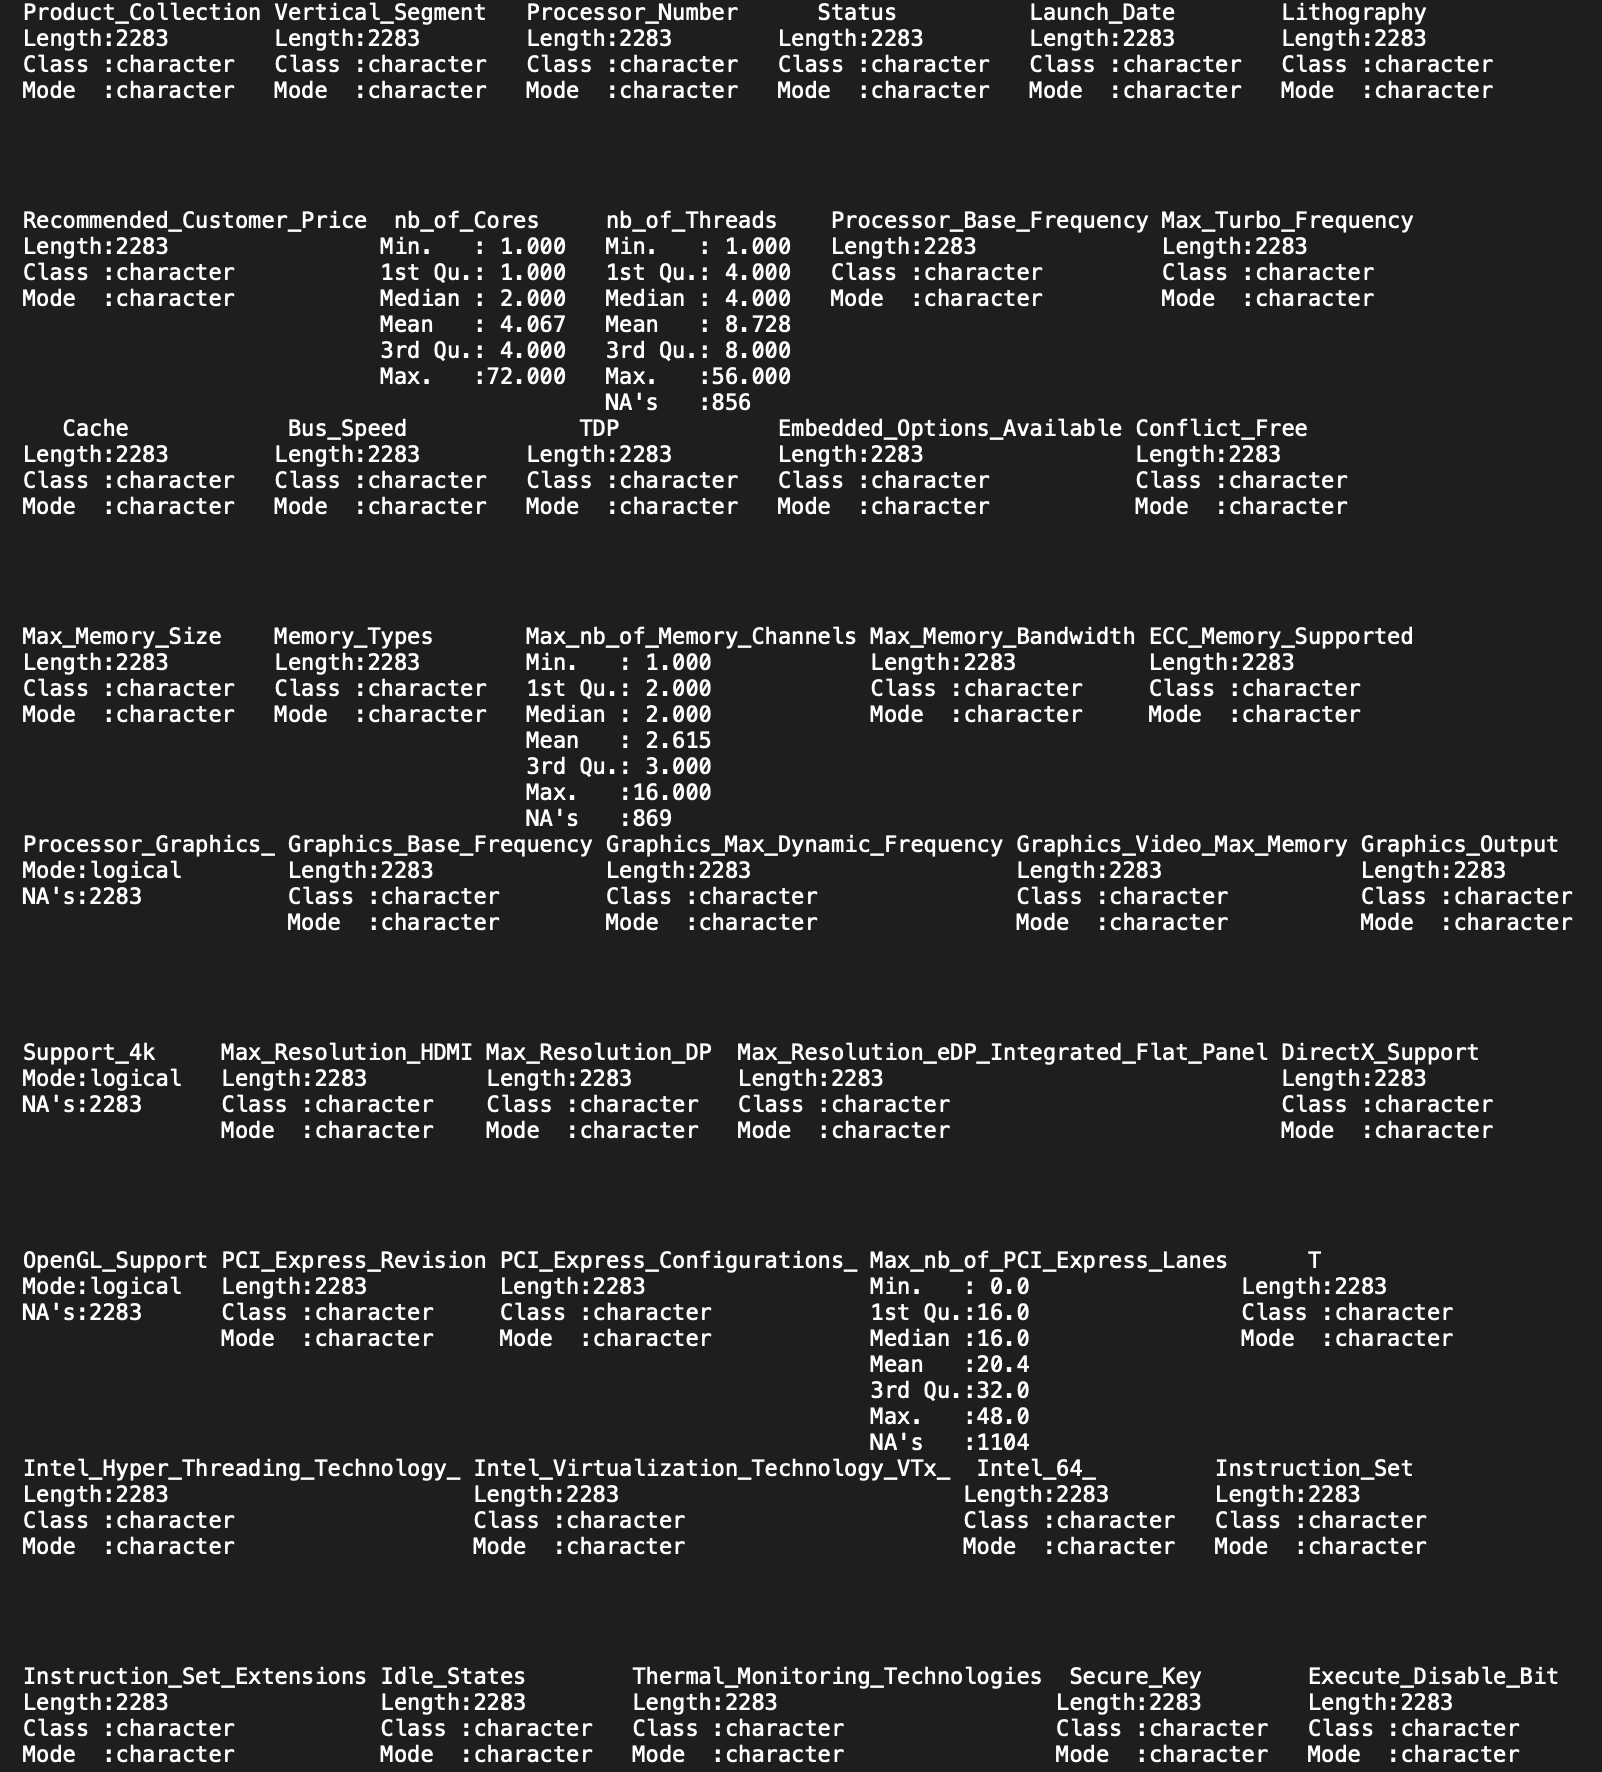
\includegraphics[width=14cm]{graphics/summary.png}
    \end{center}
\end{figure}

\subsection{Distribution and Histograms}
\begin{figure}[H]
    \begin{center}
    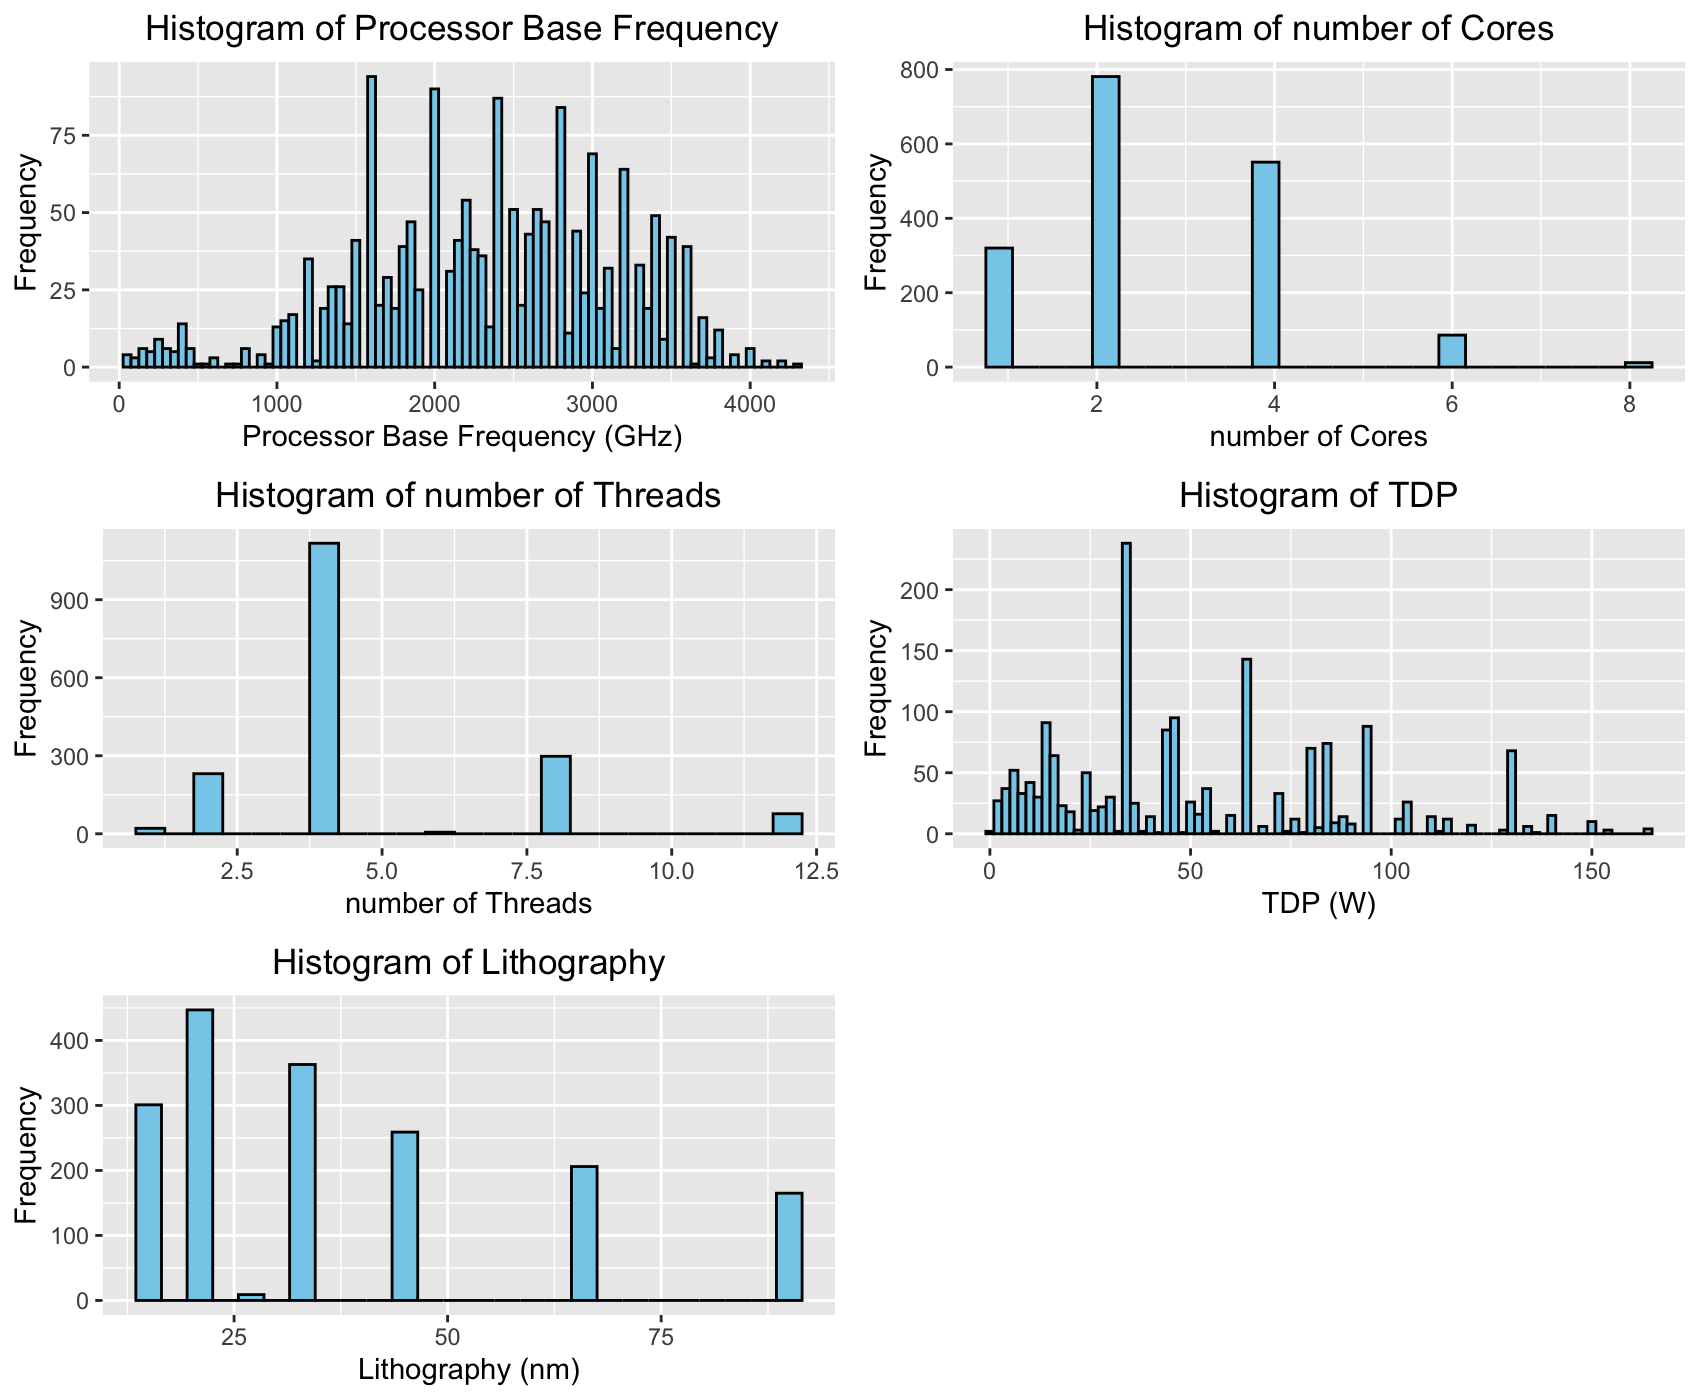
\includegraphics[width=14cm]{graphics/histogram.png}
    \end{center}
\end{figure}
\begin{itemize}
    \item Processor Base Frequency: 
    \begin{itemize}
        \item The distribution of processor base frequencies is relatively normal, with most CPUs having base frequencies between 2 and 3 GHz.
        \item A few CPUs have base frequencies below 2 GHz and above 3 GHz, indicating that while the majority of CPUs fall within a mid-range frequency, there are some outliers at both ends.
    \end{itemize}
    
    \item Number of Cores: 
    \begin{itemize}
        \item The distribution of the number of cores is right-skewed, with a large number of CPUs having between 2 and 8 cores.
        \item There are fewer CPUs with higher core counts, and very few CPUs exceed 16 cores.
        \item This suggests that while multi-core processors are common, high-core-count CPUs are less frequent.        
    \end{itemize}

    \item Number of Threads: 
    \begin{itemize}
        \item Similar to the number of cores, the distribution of the number of threads is right-skewed.
        The majority of CPUs have between 2 and 16 threads.
        \item There are some CPUs with a significantly higher number of threads, indicating the presence of high-performance CPUs with technologies like Hyper-Threading.     
    \end{itemize}

    \item TDP (Thermal Design Power):
    \begin{itemize}
        \item The distribution of Thermal Design Power (TDP) shows that most CPUs have a TDP between 50 and 125 watts.
        \item There are a few CPUs with higher TDP values, which typically correspond to more powerful processors that require more cooling.
        \item This indicates that most CPUs are designed to operate within a standard thermal envelope, but high-performance CPUs demand more power.
    \end{itemize}

    \item Lithography: 
    \begin{itemize}
        \item The lithography histogram shows several peaks, indicating different manufacturing process nodes.
        \item The most common process nodes are 14 nm and 22 nm.
        \item There are also CPUs manufactured at smaller nodes like 10 nm, and larger nodes like 32 nm and 45 nm.
        \item This reflects the advancements in semiconductor manufacturing technology, with newer CPUs being produced at smaller process nodes for improved performance and efficiency.
    \end{itemize}

\end{itemize}

Implications:
\begin{itemize}
    \item Processor Base Frequency: The relatively normal distribution suggests a common range of base frequencies, with few extreme values. This will influence our regression model, as we need to account for these outliers.

    \item Number of Cores and Threads: The right-skewed distributions indicate that while multi-core and multi-threading capabilities are common, the extent varies widely. High-core and high-thread CPUs, although fewer, represent the high-performance segment and should be carefully considered in our model.

    \item TDP: The distribution suggests that most CPUs are designed within certain power and thermal limits, but there are high-performance CPUs with higher TDP. This attribute is crucial as it impacts the CPU's ability to sustain higher clock speeds under load.

    \item Lithography: The presence of multiple peaks reflects the evolution of manufacturing processes over time. This attribute is essential for our model as newer process nodes typically allow for higher clock speeds and better efficiency.
\end{itemize}
By understanding these distributions, we can better prepare our data for inferential statistics and modeling, ensuring that our regression model accurately captures the relationship between these attributes and CPU clock speeds. This will involve handling outliers appropriately, scaling the features, and ensuring that the model is trained on a representative sample of the data.

\subsection{Boxplots for Outliers}
\begin{figure}[H]
    \begin{center}
    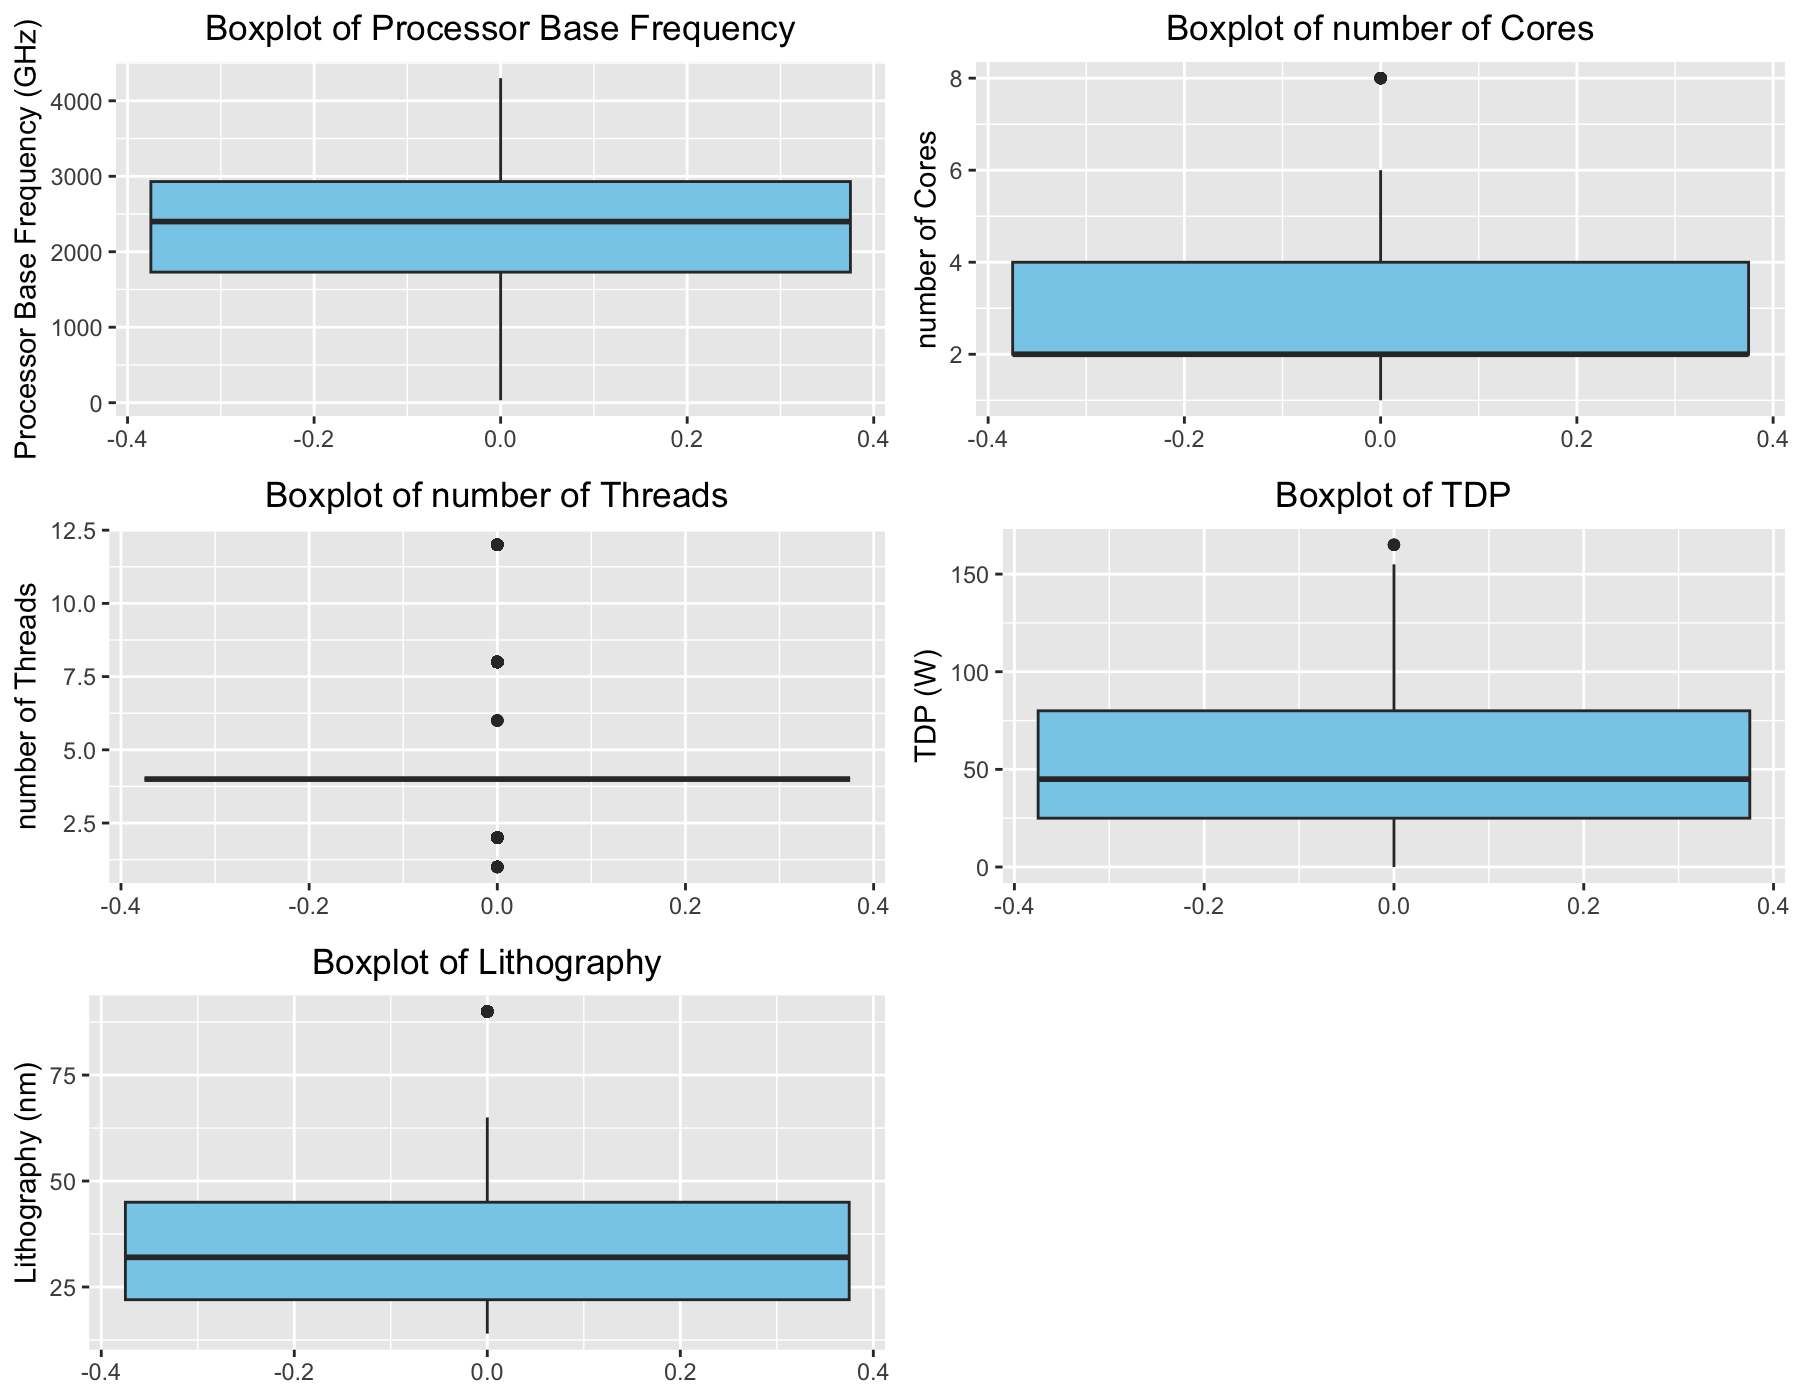
\includegraphics[width=14cm]{graphics/boxplot.png}
    \end{center}
\end{figure}
The boxplots provide a visual representation of the distribution, central tendency, and variability of key attributes in the dataset, as well as the presence of outliers. Here's a detailed explanation of each boxplot:

\begin{itemize}
    \item Boxplot of Processor Base Frequency (GHz):
    \begin{itemize}
        \item The boxplot shows the median processor base frequency around 2.5 GHz, with the interquartile range (IQR) spanning from approximately 2 GHz to 3 GHz.
        There are a few outliers above 3.5 GHz, indicating that some CPUs have significantly higher base frequencies than the majority.
    \end{itemize}

    \item Boxplot of Number of Cores:
    \begin{itemize}
        \item The median number of cores is around 4, with the IQR ranging from 2 to 6 cores.
        \item Numerous outliers are present above 8 cores, reflecting that high-core-count CPUs, while less common, are still significant.
    \end{itemize}

    \item Boxplot of Number of Threads:
    \begin{itemize}
        \item The median number of threads is around 4, with an IQR from 4 to 8 threads.
        \item There are many outliers above 16 threads, indicating that some CPUs, likely with Hyper-Threading, support a significantly higher number of threads.
    \end{itemize}
    
    \item Boxplot of TDP (W):
    \begin{itemize}
        \item The median TDP is around 65 W, with the IQR ranging from approximately 55 W to 95 W.
        \item There are several outliers below 50 W and above 125 W, showing that while most CPUs fall within a certain thermal range, some require much less or much more cooling capacity.
    \end{itemize}

    \item Boxplot of Lithography (nm):
    \begin{itemize}
        \item The median lithography value is 22 nm, with the IQR ranging from 14 nm to 32 nm.
        \item There is one outlier at 65 nm, indicating an older manufacturing process compared to the more advanced and common nodes.
    \end{itemize}
\end{itemize}

Implications:
The boxplots provide several insights that are crucial for our project on predicting CPU clock speeds:

\begin{itemize}
    \item Processor Base Frequency:
    \begin{itemize}
        \item The central tendency and spread of base frequencies are important for understanding the typical performance range of CPUs in the dataset.
        \item The presence of outliers indicates that while most CPUs have base frequencies in a common range, some high-performance CPUs exist with higher base frequencies, which need to be considered in our model.
    \end{itemize}
    
    \item Number of Cores and Threads:
    \begin{itemize}
        \item The distributions show that multi-core and multi-threaded CPUs are common, but high-core and high-thread counts are less frequent, representing high-performance segments.
        \item Outliers in these attributes reflect high-performance CPUs, which can affect the overall performance trends and must be accurately modeled.
    \end{itemize}
    
    \item TDP:
    \begin{itemize}
        \item The central tendency and variability in TDP indicate the power and thermal characteristics of most CPUs.
        \item The outliers suggest that while most CPUs operate within a standard thermal range, some require much higher or lower power, influencing their ability to sustain higher clock speeds.
    \end{itemize}
    
    \item Lithography:
    \begin{itemize}
        \item The distribution of lithography values highlights the evolution of manufacturing technology, with most CPUs produced using advanced nodes like 14 nm and 22 nm.
        \item The outlier at 65 nm represents older technology, which typically correlates with lower efficiency and performance.
    \end{itemize}
\end{itemize}

\subsection{Correlation Matrix}
\begin{figure}[H]
    \begin{center}
    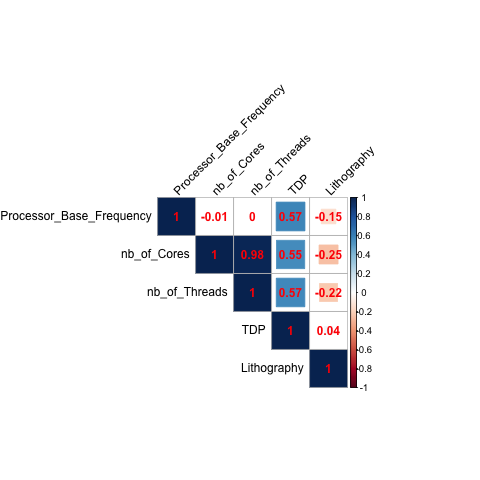
\includegraphics[width=14cm]{graphics/corr_matrix.png}
    \end{center}
\end{figure}

The correlation matrix provides a comprehensive view of the linear relationships between pairs of variables in our dataset. Each cell in the matrix represents the correlation coefficient between two variables, ranging from -1 (perfect negative correlation) to 1 (perfect positive correlation). Here's a detailed explanation of the matrix for our project:\\[6pt]
Key Observations:
\begin{itemize}
    \item Processor Base Frequency:
    \begin{itemize}
        \item Correlation with TDP: The strongest positive correlation is with TDP (0.57). This indicates that CPUs with higher base frequencies generally have higher thermal design power requirements. This is expected as higher clock speeds typically result in greater power consumption and heat generation.
        \item Negative Correlation with Lithography: There is a moderate negative correlation with Lithography (-0.15). This suggests that CPUs manufactured with smaller process nodes tend to have higher base frequencies. Advanced manufacturing technologies often result in better performance characteristics.
    \end{itemize}
    
    \item Number of Cores:
    \begin{itemize}
        \item Strong Positive Correlation with Number of Threads (0.98): This high correlation is expected as CPUs with more cores generally support more threads, especially with technologies like Hyper-Threading.
        \item Negative Correlation with Lithography (-0.25): Indicates that CPUs with a higher number of cores tend to be manufactured using smaller lithography nodes, aligning with advancements in CPU design that pack more cores into smaller spaces.
    \end{itemize}
    
    \item Number of Threads:
    \begin{itemize}
        \item Positive Correlation with TDP (0.57): Similar to the base frequency, a higher number of threads is associated with higher TDP, reflecting increased power consumption and heat dissipation needs.
    \end{itemize}
    
    \item TDP:
    \begin{itemize}
        \item Slight Positive Correlation with Lithography (0.04): This weak correlation suggests that the thermal design power does not have a strong relationship with the manufacturing process node.
    \end{itemize}
    
    \item Lithography:
    \begin{itemize}
        \item Negative Correlations with Other Variables: Lithography shows a general negative correlation with performance-related attributes, reinforcing the trend that smaller manufacturing nodes (indicative of newer technologies) are associated with higher performance capabilities.
    \end{itemize}
\end{itemize}
x
Implications:
\begin{itemize}
    \item The correlation matrix is crucial for understanding the relationships between different CPU attributes and their collective impact on clock speed. Here are some key takeaways for our project on predicting CPU clock speeds:
    
    \item TDP and Processor Base Frequency: The strong positive correlation suggests that models predicting clock speed should account for TDP as a significant predictor.
    
    \item Manufacturing Process (Lithography): The negative correlations with performance attributes highlight the importance of considering lithography advancements in performance modeling.
    
    \item Number of Cores and Threads: The strong inter-correlation indicates that either variable could be used interchangeably in some modeling contexts, but including both provides a more nuanced understanding of CPU capabilities.
\end{itemize}


\newpage
% %%%%%%%%%%%%%%%%%%%%%%%%%%%%%%%%%
\section{Inferential Statistics}
\subsection{Two-way analysis of variance(ANOVA)}
Our model is about using two-way ANOVA to determine the relationship between the dependent Processor Base Frequency with two independent which are number of Cores and Thermal Design Power(TDP). Because we want to check validity of this ANOVA model, we will have two assumption for this:\\
\\
\textbf{Normality}: Processor Base Frequency should be normal distribution for each combination of number of Cores and TDP.\\
\\
\textbf{Homogeneity}: Processor Base Frequency should be roughly across all combinations of number of Cores and TDP.
\subsubsection{Verify the assumption}
\textbf{Normality}: verify if the data is normal distribution\\
We use Shapiro-Wilk normality test to check if this model is normal distribution:\\
\\
\textbf{Null hypothesis $H_0$}: Processor Base Frequency should be approximately normally distributed for each combinations of number of Cores and TDP.\\
\\
\textbf{Alternative hypothesis $H_1$}: Processor Base Frequency should not be approximately normally distributed for each combinations of number of Cores and TDP.
\begin{figure}[H]
    \centering
    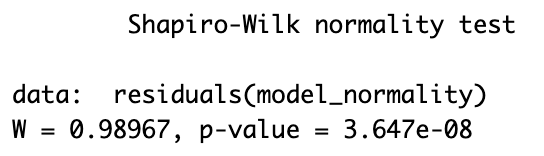
\includegraphics[width=0.8\textwidth]{graphics/shapiro.png}
    \caption{Shapiro-Wilk's test}
    \label{fig:shapiro}
\end{figure}
From the result, p-value is smaller than 0.05 so we reject $H_0$ and accept $H_1$. Therefore, Processor Base Frequency should not be approximately normally distributed for each combinations of number of Cores and TDP. So we need to plot out the model diagnose plot to check if it is normal distribution or not:
\begin{figure}[H]
    \centering
    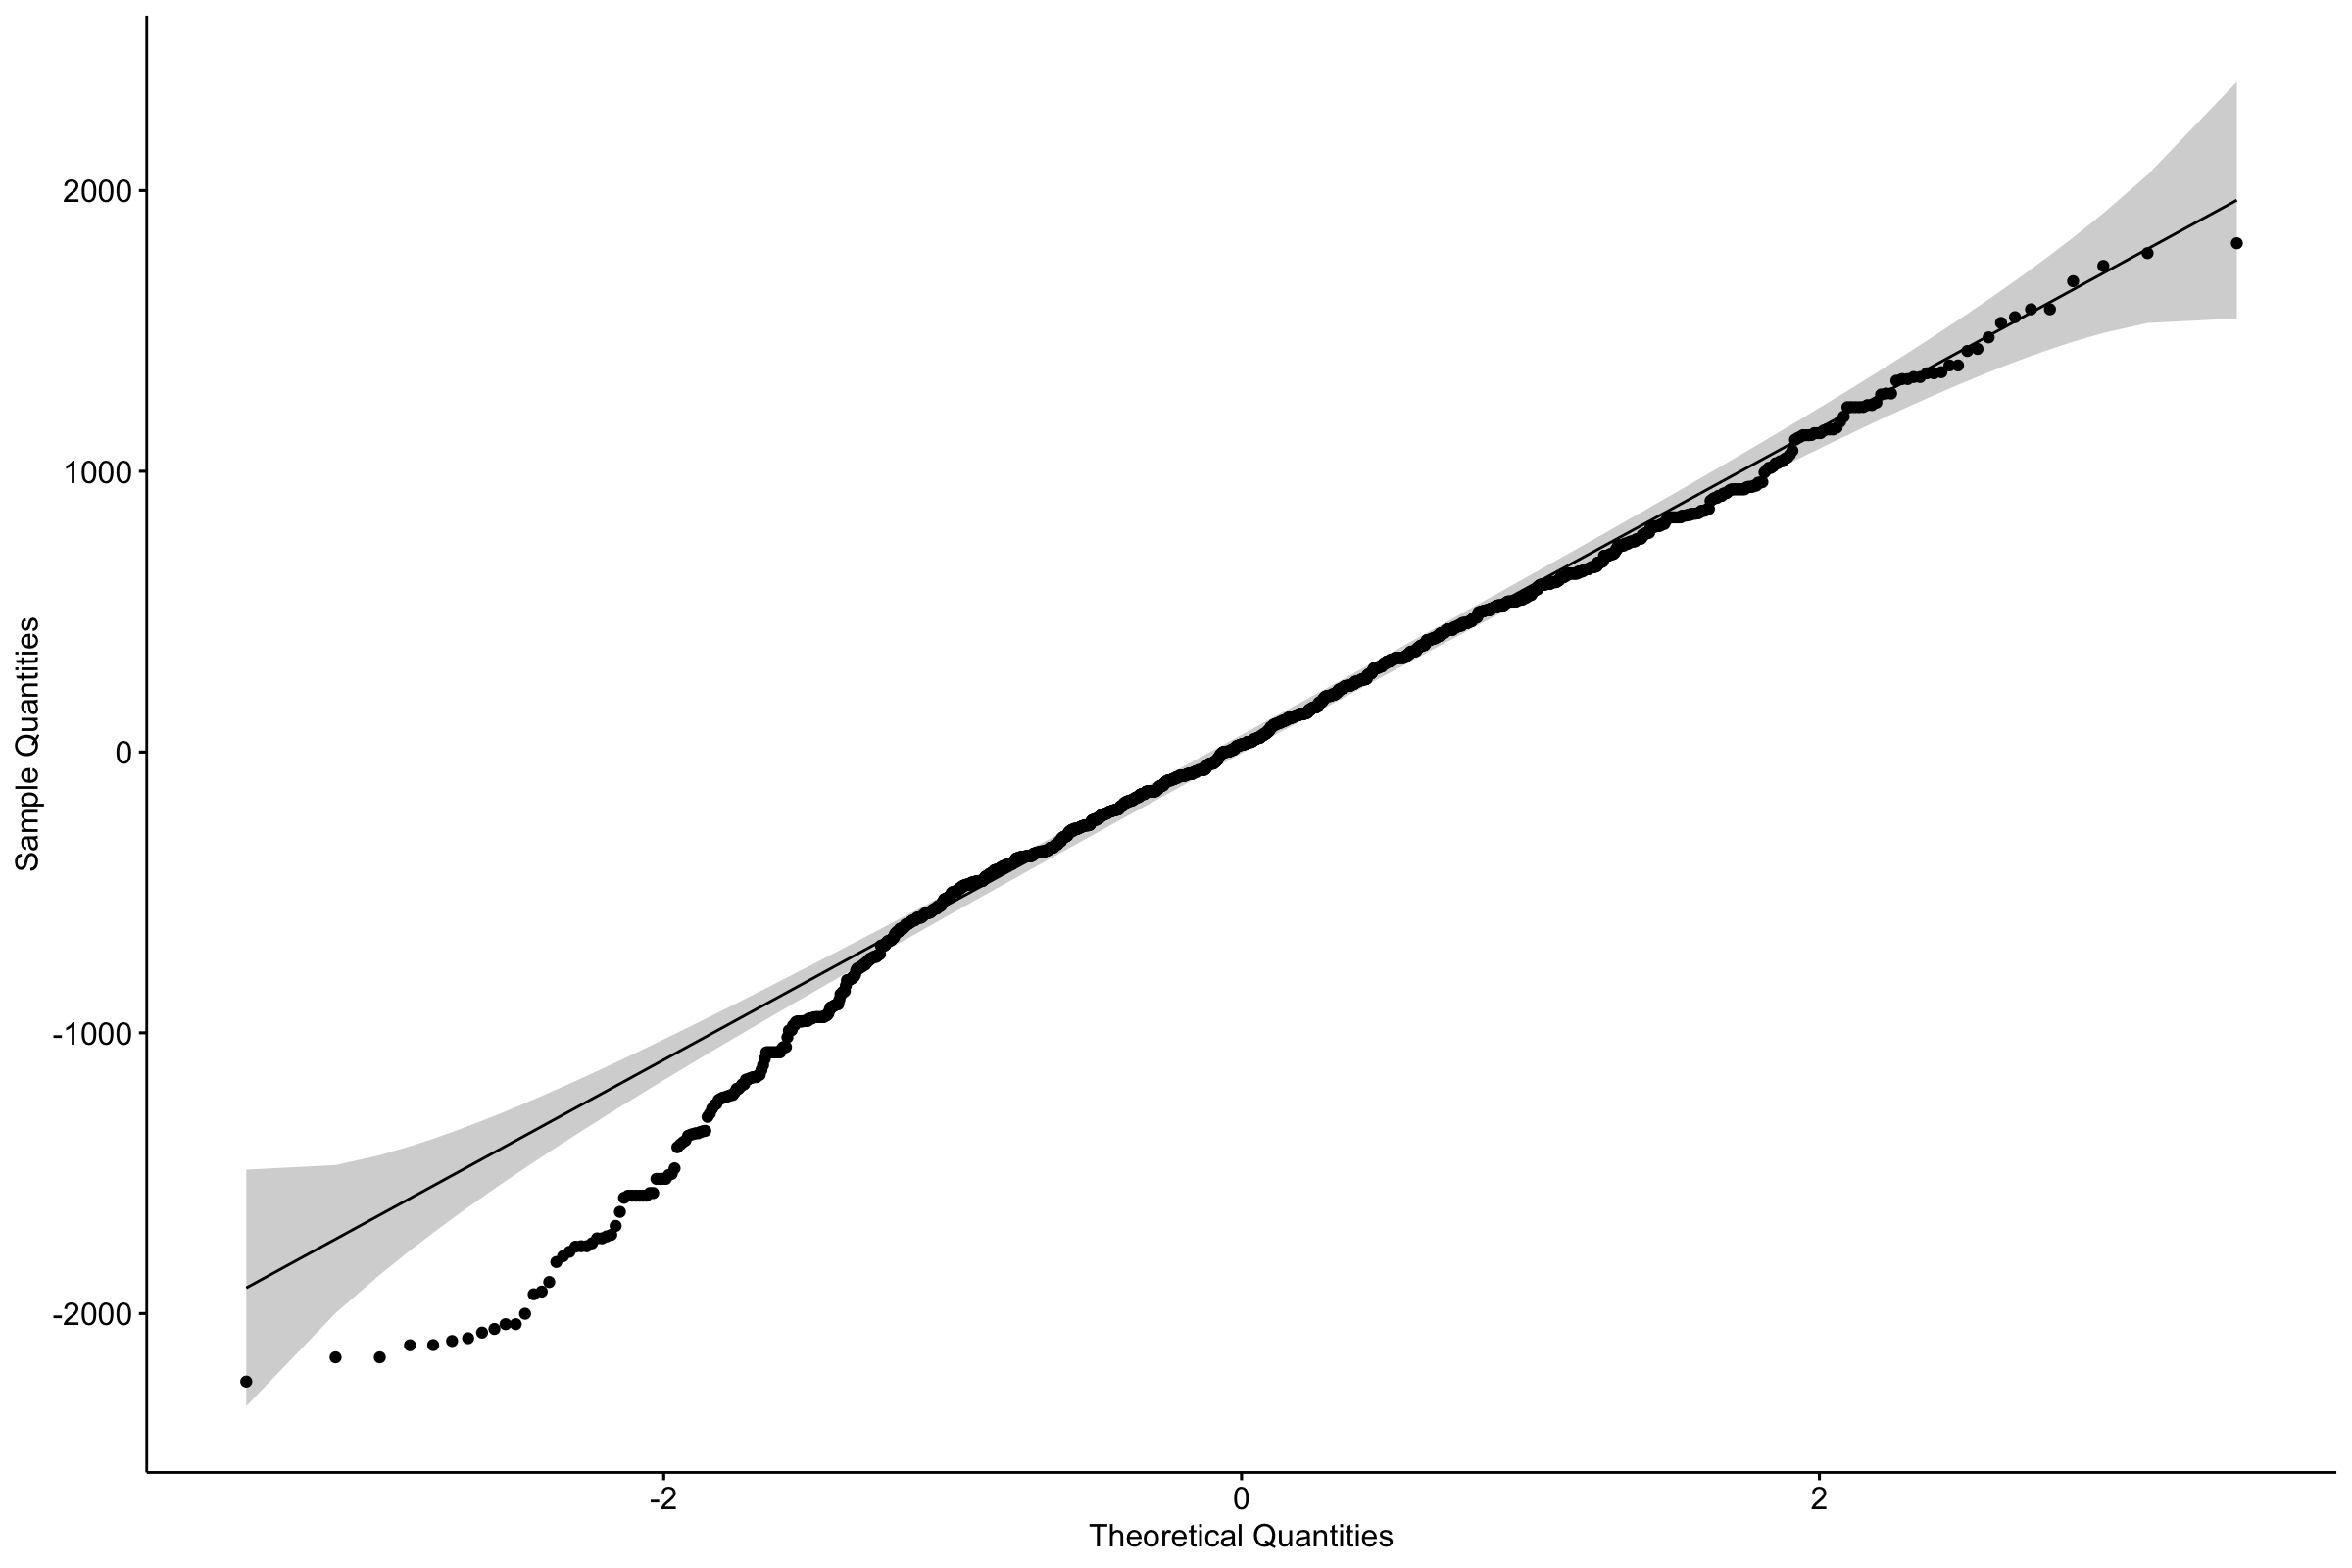
\includegraphics[width=1\textwidth]{graphics/check_normality.png}
    \caption{ggqqplot from ANOVA test}
    \label{fig:check_normality}
\end{figure}
We see that in ggqqplot, most of the points lie closely on the line. So we can assume that Processor Base Frequency is approximately normally distributed for each combinations of number of Cores and TDP.\\
\\
\textbf{Homogeneity}: verify the uniformity of the variance.\\
\\
We use Levene's test to check if this model is homogeneity:\\
\\
\textbf{Null hypothesis $H_0$}: Processor Base Frequency is homogeneity across groups of number of Cores and TDP.\\
\\
\textbf{Alternative hypothesis $H_1$}: Processor Base Frequency is not homogeneity across groups of number of Cores and TDP.
\begin{figure}[H]
    \centering
    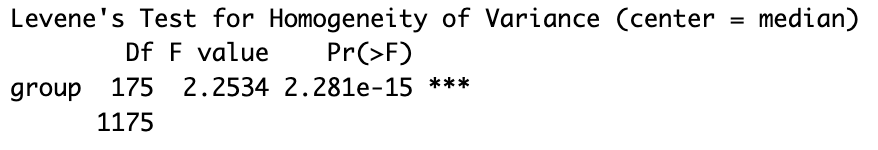
\includegraphics[width=1\textwidth]{graphics/check_homogeneity.png}
    \caption{Leneve's Test for Homogeneity of Variance}
    \label{fig:check_homogeneity}
\end{figure}
From the result, we see that p-value is smaller than 0.05 so we reject $H_0$ and accept $H_1$. Therefore, Processor Base Frequency is not homogeneity across groups of number of Cores and TDP. 
\subsubsection{Calculate ANOVA}
\textbf{Null hypothesis $H_0$}: Processor Base Frequency follows the same distribution across group defined by the independent variables number of Cores and TDP.\\
\\
\textbf{Alternative hypothesis $H_1$}: Processor Base Frequency follows different distribution across group defined by the independent variables number of Cores and TDP.
\begin{figure}[H]
    \centering
    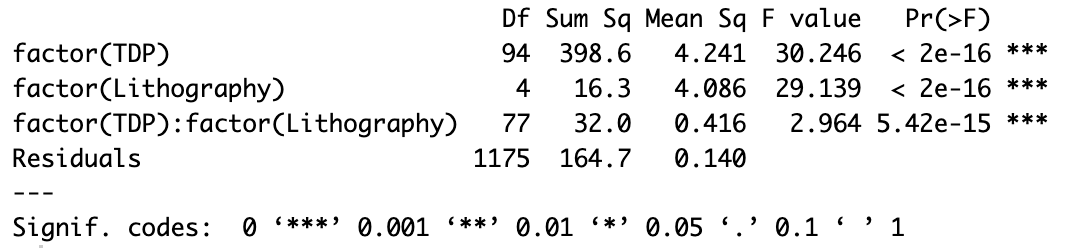
\includegraphics[width=1\textwidth]{graphics/anova_test.png}
    \caption{Calculate ANOVA}
    \label{fig:calculate_anova}
\end{figure}
From the result, we see that Pr(>F) value is smaller than 0.05 so we reject $H_0$ and accept $H_1$. Therefore, Processor Base Frequency follows different distribution across group defined by the independent variables number of Cores and TDP.

\subsection{Multiple Linear Regression to Predict CPU Clock Speed}

\subsubsection{Data Splitting}
After finalizing the data we need for statistical analysis, we have to split the data further into two subsets: \textbf{training set and test set}. Training set helps us build and train the model, allowing it to learn the patterns and connections within our data. Then, the test set will be tested on the validated model to give an objective assessment of the model's efficacy and performance on fresh, unseen data. In data science and machine learning, this train-test split strategy is a standard procedure since it ensures that the model generalises effectively to new data and helps prevent over-fitting. In this project, the training set consists of 70\% of the original data, and the remaining 30\% makes up the test set.

\subsubsection{Regression Model}
The main objective of this section is constructing a model that portrays the effect of other factors on the CPU clock speed. To achieve this we applied a Multi Regression model, in which the dependent variable is Processor Base Frequency - the variable representing CPU clock speed, and the rest are independent. Our model appears as the formula below:\\

$Processor Base Frequency = \beta_0 + \beta_1 nb\_of\_Cores + \beta_2 nb\_of\_Threads + \beta_3 TDP + \beta_4 Lithography$ \\

We start with our \textbf{first model}, also known as the \textbf{base model}, built with all the independent variables available. \\

%ảnh model 2

In this model, our respone variables consist of: nb\_of\_Cores, nb\_of\_Threads, TDP and Lithography. Now, we should remove the variables that are proven insignificant to our analysis, which can be determined based on the Pr values (last column). If $Pr < 0.05$, the variable is significant. With this insight, the variable that will be deducted is nb\_of\_Threads. Subsequently, we now construct the \textbf{new and theoretically improved model}. \\

%ảnh model 3

However, our group came to the decision of using the base model, since the difference in Adjusted $R^2$ value between the two is not significant enough (0.0001) to implement the second model as an improvement over the first. Hence, our final model now should look like this:\\

$Processor Base Frequency = \beta_0 + \beta_1 nb\_of\_Cores + \beta_2 nb\_of\_Threads + \beta_3 TDP + \beta_4 Lithography$ \\

Observing the results R gave on model 2, the p - value correlating with F statistics is less than $2.2 \cdot 10^{-16}$. This suggests that our data is robust and valuable for statistical analysis. Additionally, it guarantees that future results from this model provide good evaluations about the relationship between the Processor Base Frequency and the remaining variables. Generally, the regression coefficients ($\beta_i$) and the p - values hold the most influences on the independent variables. 

\subsubsection{Assumptions of Linear Regression}

\subsubsection{Testing}
We now use the preceding test set to access the accuracy of our model. To gauge the correspondence between our estimates and the actual values, we look at their distribution and compare them.

%plot và bảng so sánh 2 data set

Khúc này là nhận xét nhma đ có data gì nên chưa nhận xét nha bây :')

\subsection{Conclusion}
After implementing a Multi Regression Model to predict the CPU Clock Speed, we were able to identified 4 variables that are significant to the Processor Base Frequency. The model aid manufacturers in pinpointing the factors that affect the CPU performance through its clock speed, providing appropriate strategies in product development, while also help customer choosing the right CPU specifications for their needs. Overall, the results that the model predict is justifiably similar to the actual data. 

\newpage

% %%%%%%%%%%%%%%%%%%%%%%%%%%%%%%%%%
\section{Conclusion}

\newpage
% %%%%%%%%%%%%%%%%%%%%%%%%%%%%%%%%%
\clearpage
\section{References}
\bibliographystyle{unsrt}
\bibliography{citations/books.bib}
\nocite{*}

\end{document}